To test both \acrshort{fer} and \acrshort{ser} in real-world scenarios, the trained models will be embedded in a pipeline to allow us to apply the trained model on real-world captured images and speech recordings. For \acrshort{fer} this can then in turn be applied to frames of a video, that will be captured by a camera, evaluating the emotions of one person (possibly multiple people if feasible). Accordingly, for \acrshort{ser} the users' utterances will be recorded with a microphone. Hereby, the continuous audio stream should then be cut every $x$ seconds to obtain the data samples. As Figure \ref{fig:whole-system} shows, both inputs will be preprocessed and fed into the respective models. The results from both of the approaches will then be continuously published on the user interface. Here, the users indicate whether one or both of the classifications are correct by stating their actual emotion through a small GUI. The user feedback will be stored along the respective image and audio sample and can then be used to retrain the model with more data, if the accuracy drops below a predetermined threshold. Overall, we aim to develop a robust and accurate combined system for facial and speech emotion recognition that can be applied to a range of real-world applications.

\begin{figure}[h]
\centering
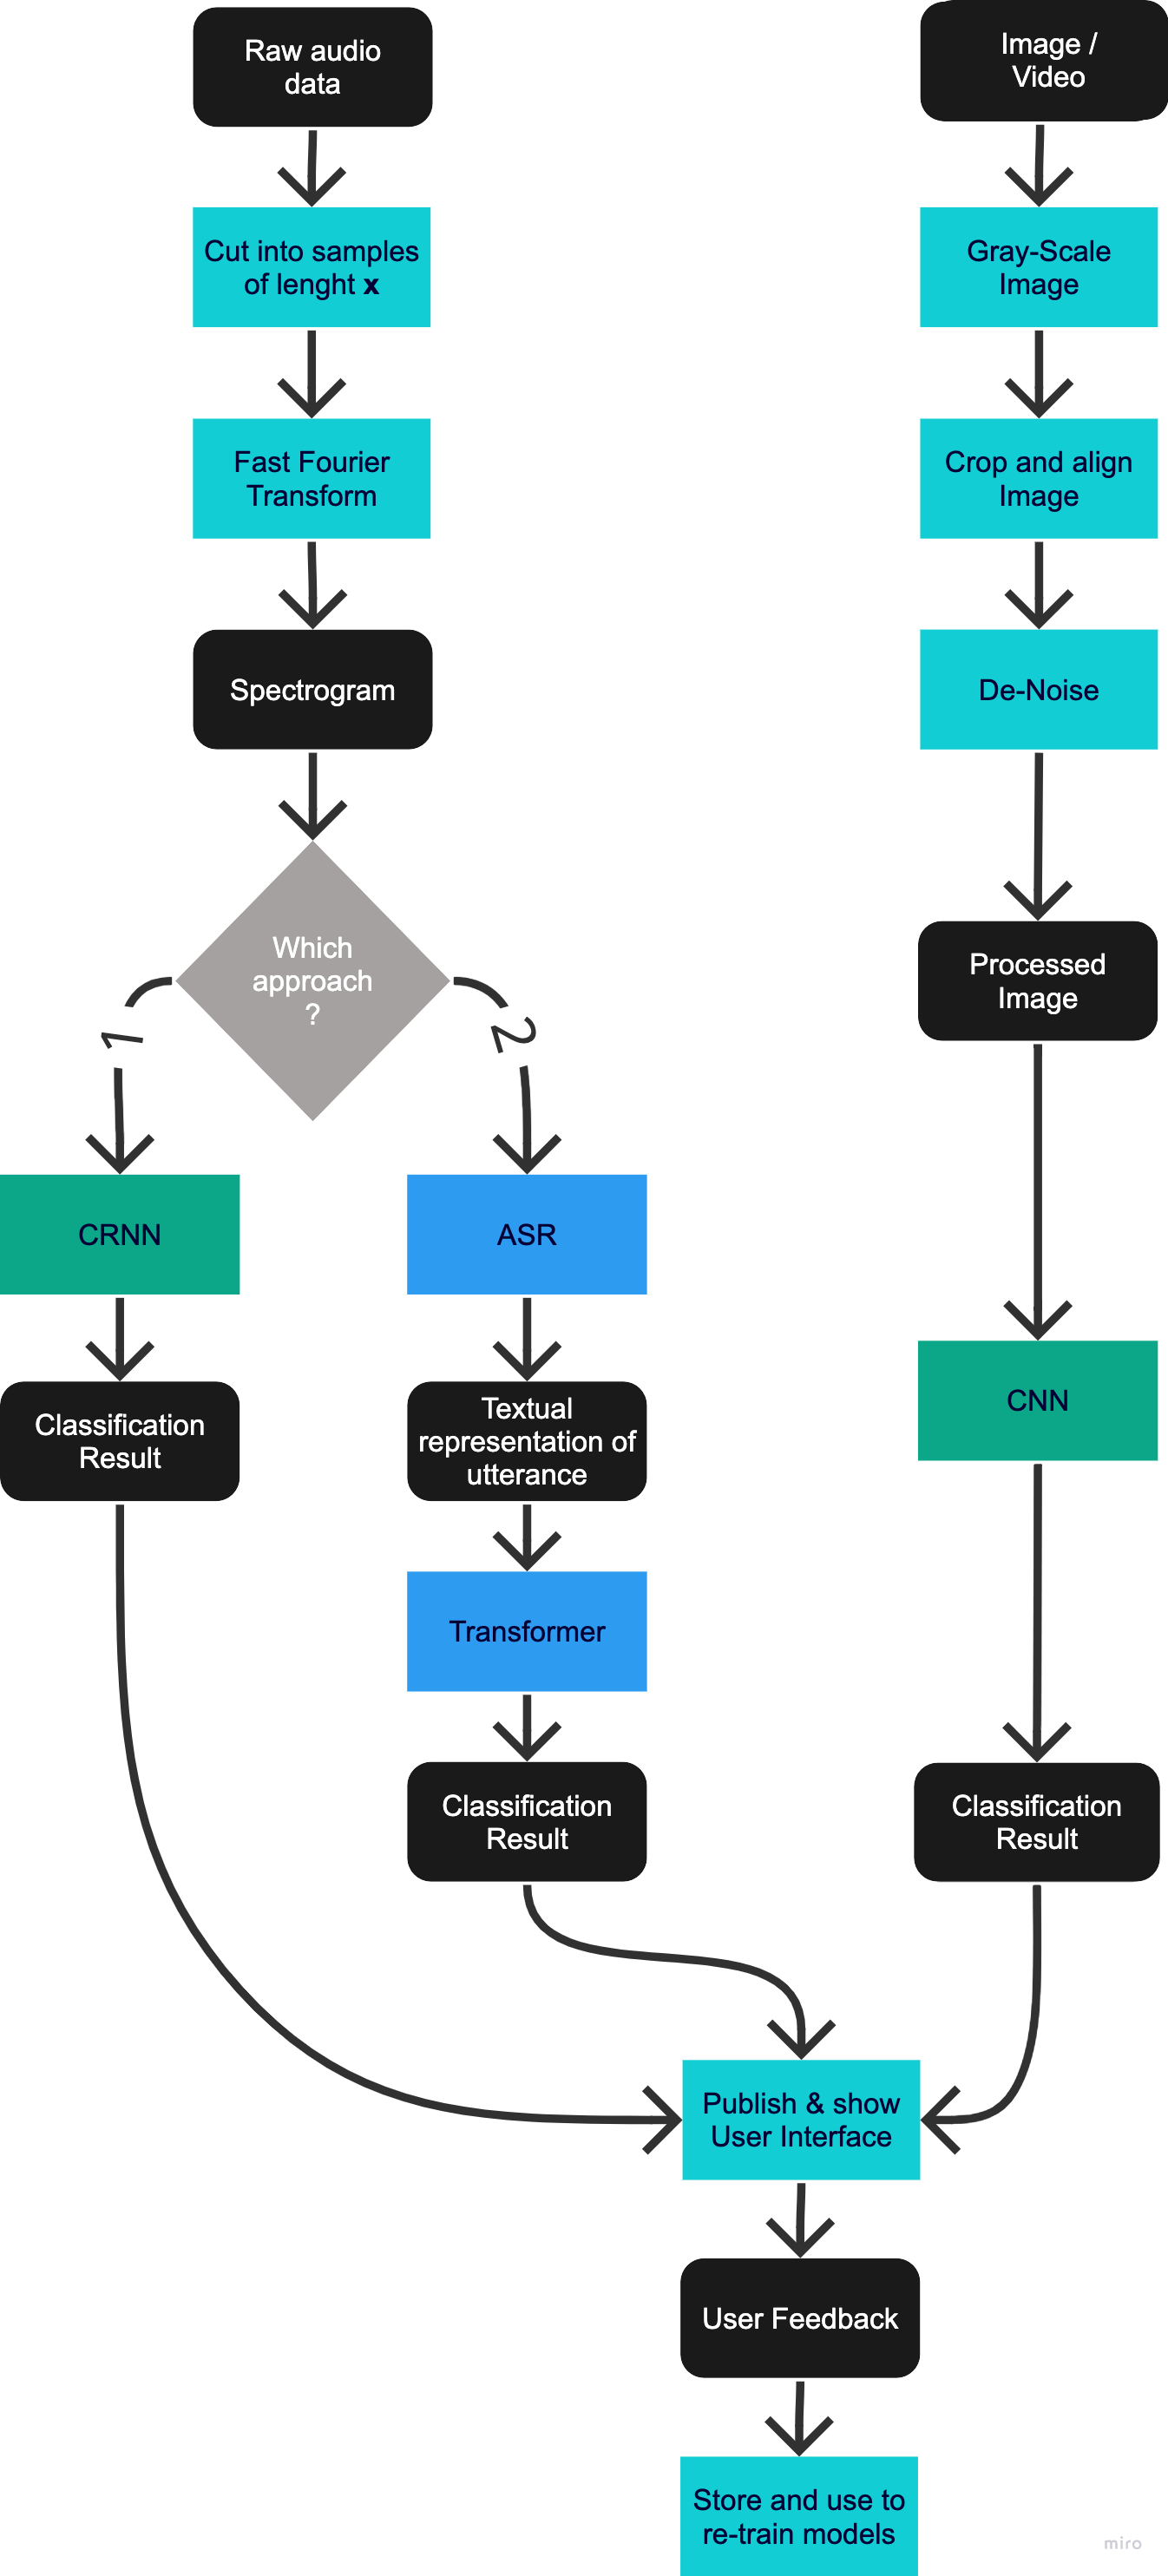
\includegraphics[width=0.7\textwidth]{images/whole-system.png}
\caption{Structure of the entire system}\label{fig:whole-system}
\end{figure}